\label{ch:design}

introduction



\section{Bottom-up Abstraction}



\section{Refining the properties}
This section describes how the properties generated from the master agent and bus matrix PPAs are refined to hold on the design. Before we delve into the specifics of the refinement, some key aspects of the generated properties are introduced. \par

\subsubsection{Signal macro}
Every I/O signal and variable of the design is represented with a signal macro. Every signal macro is of the form: \par
\ITLKW{macro} signal\_name : \ITLIW{type} := refinement \ITLKW{end macro}; \par

The I/O signals are divided in two categories; DP signals and sync/notify. Sync/notify is a set of macros representing the event signaling of the blocking interface. Every blocking port has exactly one sync (input), one notify (output) and a set of DP signals corresponding to the size of the payload. The DP signals can go either direction, but will normally correspond to the direction of the port it represents. The DP signals of a blocking port are not listed in the commitment part of a property unless its corresponding notify is set. Shared ports are only represented through DP signals.\par
Every variable which is read in a different state than it was written, is represented with a signal macro. These signal macros are referred to as visible registers. They carry information between the states/properties. \par
The final set of signal macros are the states, which always have boolean type. The amount of states of the generated properties can be higher than the excplicit states defined in the SystemC-PPA. This is the case of the bus matrix, where the communication over each blocking port is represented with its own state macro, as well as any states inserted with the \textit{instert\_state()} command. Following is an example of how to refine each of the described macros: \par
\ITLCOMMENT{macro bus\_to\_slave\_notify0 : \ITLIW{boolean} := end macro;} \\ 
Sync and notify signals often have the same name and function as in the RTL model, they are removed. \par
\ITLKW{macro} bus\_to\_slave0\_sig\_hwdata : \ITLIW{unsigned} := bus\_to\_slave0.hwdata \ITLKW{end macro}; \\
DP signals are often mapped directly to the similarily named RTL signal they represent. \par
\ITLKW{macro} addr\_own : \ITLIW{unsigned} := matrix/ahb\_arb0/master\_sel \ITLKW{end macro}; \\
Visible register mapped to lower level physical register. \par
\ITLKW{macro} slave\_agent0\_writes\_out : \ITLIW{boolean} := bus\_to\_slave0\_notify \ITLKW{end macro}; \\
State macro refined to be true when a certain notify is set. \par
This covers the essentials to follow the refinement of the properties in this work. The refinement process focuses on the signal and state macros. 

\subsection{Master Agent}
The macros representing the signals of the master agent are mostly mapped directly to the similarily named top level RTL signal they represent. The exceptions are described in turn, beginning with the signals related to the emulated port. \par

\begin{VHI}
macro bus_ready_sync : boolean := bus_to_mAgent0.hready end macro; 
macro bus_ready_notify : boolean := 
master_stage = Data or master_stage = Address
end macro;
macro bus_ready_sig : boolean := true end macro; 
\end{VHI}

\ITLKW{macro} bus\_ready\_sync : \ITLIW{boolean} := bus\_to\_mAgent0.hready \ITLKW{end macro}; \\
\ITLKW{macro} bus\_ready\_notify : \ITLIW{boolean} := \\
master\_stage = Data \ITLRW{or} master\_stage = Address\\
\ITLKW{end macro};\\
\ITLKW{macro} bus\_ready\_sig : \ITLIW{boolean} := \ITLKW{true} \ITLKW{end macro}; \par

Three signal macros are generated for the port representing \textbf{HREADY}. Only the input, \textit{sync} is refined to the corresponding signal in the RTL description, the others are given arbitrary abstract values that satisfy the properties. There are no outputs that explicitly signals that the agent is waiting for the bus to be ready. \par

\ITLKW{macro} mAgent\_request\_sync : \ITLIW{boolean} := \\
bus\_to\_mAgent0.hready \ITLRW{and} bus\_to\_mAgent0.hgrant \\
\ITLKW{end macro}; \\
\ITLKW{macro} mAgent\_request\_notify : \ITLIW{boolean} := mAgent\_to\_bus0.hbusreq \ITLKW{end macro};\\
\ITLKW{macro} mAgent\_request\_sig : \ITLIW{boolean} := mAgent\_to\_bus0.hbusreq \ITLKW{end macro}; \par

Three signal macros are generated for the port representing \textbf{HBUSREQx}, which all can be refined to actual inputs and outputs.  The DP signal of this port; mAgent\_request\_sig is technically redundant. \par 

The DP signal represeniting data size is represented with an enum at the ESL, which is refined as follows to satisfy the properties: \par
\ITLKW{macro} mAgent\_to\_bus\_sig\_hsize : mask := \\
\ITLKW{if}(mAgent\_to\_bus0.hsize = \ITLRW{"000"}) \ITLKW{then} MT\_B \\
\ITLKW{elsif}(mAgent\_to\_bus0.hsize = \ITLRW{"001"}) \ITLKW{then} MT\_H\\
\ITLKW{else} MT\_W \\
\ITLKW{end if}; \\ 
\ITLKW{end macro}; \par


\section{RTL design and configuration}

\subsection{Packages and configuration files}


\subsection{Designing Agents In RTL}
The master and slave agents translates a payload to and from a message passed according to the AHB protocol respectively. The agents must comply with the protocol, which can be manually verified. In this work, the protocol is verified in three ways. The simulation waveforms are compared to the specification and formal properties show that the payload reaches its target. The final method is to connect a slave to the system from an external source. The choice of this is the AHB3Lite\_memory \cite{ahbmen}. The master agent writes a message to a memory address and checks that it can successfully retrieve this message. 

\subsubsection{Master Agent}



\subsubsection{Slave Agent}


\subsection{Putting it together}



\section{ESL design}

\subsection{Bus matrix}

\subsection{Master agent}

\subsection{Emulated port}





\section{Simulation}
\label{sec:sim}
Simulation models carrying out the same operations are designed for both abstraction layers. One of the main benefits of modeling hardware at the ESL is simulation speed, so a time comparison is carried out between the two layers. Designing two corresponding simulation models also offers some verification. 
The aim of PDD is to do away with RTL simulation altogether, but when the ESL description is modeled after an existing hardware architecture it makes sense
to ensure that the two simulation models behave equally. \par
Master and slave dummies are connected to the bus matrix. The master dummy can not tell if the response it got originated from the slave it intended to communicate with. The slave dummies do not know their address offset, or which master initiated the transfer. It is possible to implement a monitoring procedure at the ESL by utilizing the high level capabilities of C++. VHDL do not offer the same capabilities and to ensure equality in both simulation models, a different approach is used. The master dummy alternates between single read and writes. For every write transfer, it encodes an identification number into the data. It is simply done by adding the ID of the slave it intends to access to the top 8 bits of the data payload. The slave asserts that the ID encoded in the data matches its own, which verifies that the intended slave is accessed. \par
For every read transfer, the slaves response data is its ID. The master asserts that the ID in the response data matches the address of the transfer it initiated, which verifies that the correct master receives the response data. This proof is vacuous if all masters access the same slave at all times, but any errors are detected when the masters cross slave address boundaries. The simulation lasts for the duration of $10^6$ transfers, during which the address wraps around to 0 if it reaches the end of the slave address range. Accessing the default slave does not increment the transfer count, so choosing a non continuous address range will affect the simulation time.
  

\subsection{Starvation}
One drawback of fixed-priority arbitration is that lower priority masters may never be granted access to the bus. When this occur depends on the amount of masters, the rate of transfer for each master and the duration of each transfer. It can be observed from RTL simulation that a fourth master is never granted access if all three higher priority masters request the bus as rapidly as allowed by
the implementation. It is not possible for an untimed ESL simulation to exactly reflect such time dependent behavior. What is important to accurately reflect in the ESL simulation is whether a master starves forever or not. \par
In the provided test bench this is modeled accurately because it is easy to observe the differences in the simulation types. If all masters request out of range it is the fifth master, rather than the fourth that starves forever. This is because the default slave responds faster and the delay between the agents response to a new request is at least three clock cycles. The fourth master is in this case granted the bus before the first master has time to request anew. There exists no such delay at the ESL, so the fourth master is never granted access here unless delay of $3*MIN\_WAIT\_TIME$ is added and $MIN\_WAIT\_TIME>0$. \par
It is not a real scenario that all masters request out of range forever, but it highlights an issue with untimed models and starvation. It is safe to say that a fourth and fifth master will at some point be granted access to the bus, because all masters will not always request access. When a system contains a high number of masters that request access to the bus at varying rates, a $3*MIN\_WAIT\_TIME$ delay inserted is likely not enough to ensure equivalent simulation behavior. \WKSAY{is the only option here a better arbitration protocol?}


\section{Experimental results}
\label{sec:results}

\begin{table}[hbt] 
  \label{tab:stats}
  \begin{tabular}{ l r r r r r}
  \hline 
  \hline
      & \multicolumn{2}{c}{\textbf{\_\_\_}RTL\textbf{\_\_\_}} & \multicolumn{3}{c}{\textbf{\_\_\_\_\_\_}PPA\textbf{\_\_\_\_\_\_}} \\
  Modules & inp./out. & FFs & inp./out & var. & states/ops \\
    \hline
  Master agent & 107/114 & 107 & 2/4 & 8 & 5/11 \\
  \hline
  Bus matrix & - & 114 & 1/1 & 13 & 4/$(17+4m)s$* \\
  
  Per slave & 107/114 & 193 & 1/1 & - & 4/- \\
 
  Per master & 106/47 & 111 & 1/1 & - & -/- \\
    \hline
    \hline  
  \end{tabular}
\caption{AHB resource comparison}
\end{table}


\begin{table}[hbt] 
  \label{tab:stats}
  \begin{tabular}{ r r r r }
  \hline 
  \hline
    N.o.mst.  & N.o.slv. & RTL & ESL \\
    \hline
      1 & 1 & 232s & 7s \\
  
      2 & 1 & 178s & 6s \\
  
      1 & 2 & 250s & 7s \\
 
      3 & 1 & 115s & 6s \\

      1 & 3 & 257s & 7s \\

      3 & 2 & 120s & 7s \\
 
      2 & 3 & 197s & 7s \\

      3 & 3 & 129s & 7s \\

      6 & 6 & 130s & 7s \\

      9 & 9 & 153s & 7s \\

      12 & 12 & 180s & 7s \\

      15 & 15 & 195s & 7s \\

      15 & 5 & 150s & 7s \\

      5 & 15 & 174s & 7s \\
    \hline
    \hline  
  \end{tabular}
\caption{Simulation of $10^6$ transactions}
\end{table}

9m9s RR: 135s, 70000060ns FP 153s, 70000120ns
12m12s RR: 152s
15m15s RR: 175s
15m5s  RR: 133s
5m15s  RR: 158s
3m15s  RR: 193s    FP: 178s





\section{Concept: Burst Transfer}
\label{sec:burst}
A big part of the AHB specification is dedicated to burst transfers. The implementation of burst transfers with SystemC-PPA is explored in this work, and a proof of concept is developed. 
This proof of concept involves a four beat incremental burst transfer, which can not be terminated early. This section elaborates on the implementation of this proof of concept. The functionality
of the four beat incremental burst is first implemented in the master and slave agents at the RTL, where compliance with the protocol is thoroughly verified with waveform simulation. The ESL model is
modified to model the four beat incremental burst, where functionality is checked with simulation. Finally, property sets are generated from the ESL model and refined to hold on the RTL design. For this proof of concept, a system with a single master and slave is used. 

\subsection{RTL}
The open source bus matrix RTL needs no modification, as it already supports all burst transfers. An additional state is added to the state machine of both agents, \textit{Addr\_Data}. 

\begin{figure}[hbt]
 \centering
 \begin{subfigure}[b]{0.3\linewidth}
 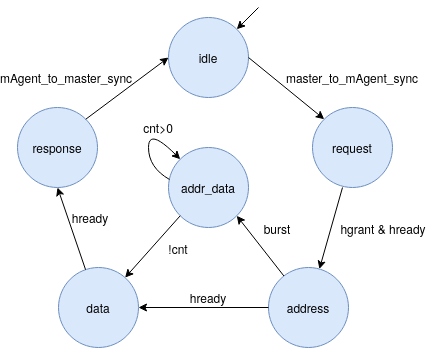
\includegraphics[width=\linewidth]{figs/hw/mAgent_burstfsm.png}
 \caption{Master agent}
 \end{subfigure}
 \begin{subfigure}[b]{0.3\linewidth}
 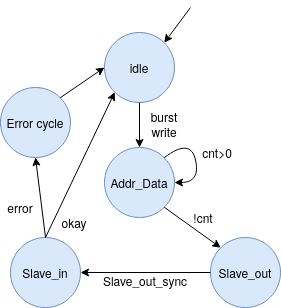
\includegraphics[width=\linewidth]{figs/hw/sAgent_wburstfsm.png}
 \caption{Slave agent burst write}
 \end{subfigure}
 \begin{subfigure}[b]{0.3\linewidth}
 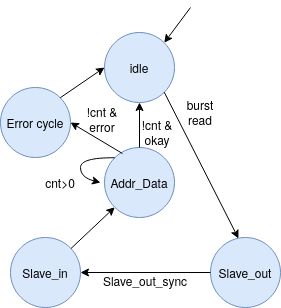
\includegraphics[width=\linewidth]{figs/hw/sAgent_rburstfsm.png}
 \caption{Slave agent burst read}
 \end{subfigure}
\label{fig:burst-fsm}
\end{figure}

Fig.~\ref{fig:burst-fsm} show the finite state machines with burst transfers added. Single read and write has been removed from the slave agent FSMs for visibility, they still function as shown in Fig.~\ref{fig:rsfsm}. Furthemore, the burst read and write is shown in separate figures to avoid confusion with regards to the transitions. 

\subsubsection{Master Agent}
The master agent receives a burst request from its master. If the transaction is a write, data is loaded into a write shift register. The agent continues through the \textit{Request} and \textit{Address} state as usual. In the \textit{Addr\_Data} state, data is either clocked out on \textbf{HWDATA} from the write shift register, or clocked in to the read shift register from \textbf{HRDATA}, when the bus is ready. Data sizes are limited to word size only in this proof of concept, so address is simply incremented by four. The burst transaction ends in the state \textit{Data}, where valid data is maintained on \textbf{HWDATA} until the bus is ready, or sampled from \textbf{HRDATA} when the bus is ready. The transaction ends with the read shift register being written to the master, along with status of transfer. There is no mechanism implemented to enable early burst termination, a "fair" arbitration policy must be used. If an error is received mid-transfer the remaining beats of the transfer are carried out. 

\subsubsection{Slave Agent}
The slave agent detects that the initiated transfer is a burst transaction. If it is a write transaction it clocks in all data and addresses into shiftregisters. The slave agent drives \textbf{HREADY} low as the final data is received, to extend the transfer until it has communicated the request to its slave. The transfer is completed when the slave responds with status. \par
If the transaction is a read, the slave samples the first address and drives \textbf{HREADY} low to communicate the request its slave. When the slave responds, response data is clocked out on a response shiftregister while address is clocked in. The transfer is completed when the final beat of the burst is clocked out. If the status of the burst read is error, data and address are still clocked out and in respectively, but the two cycle error response finalizes the transfer.  


\subsection{ESL}
Modifications are made to the master agent, bus matrix and emulated port. The burst transfers are modeled using blocking ports and some helper variables. The burst transfer payloads are routed through the emulated port, whereas single transfers proceed as usual.

\subsubsection{Emulated port}
\begin{wrapfigure}[12]{l}{5.5cm}
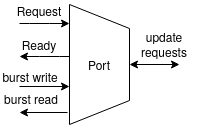
\includegraphics[width=5.5cm]{figs/ESL/em_port_burst.png}
\caption{Modified port connections}\label{fig:em-burst}
\end{wrapfigure}

The request port is modified from a boolean to a helper payload, which is used by the port to determine transfer type, first address and transfer write data. The added burst ports are connected to the master agent. The burst read and write port each transfer burst payloads. These payloads contain all address and data words and control signals which will be communicated in the four beat burst. The port \textit{update\_requests} is modified from boolean to a burst read payload from the bus matrix. Shared out ports containing address and write data is added between the port and the bus matrix. An overview of a write burst transaction is provided, each stage starts and ends at the port \textit{update\_requests}:

\begin{enumerate}
 \item The emulated port fetches the burst helper payload from the request port, and bus access is requested as usual.
 \item The address from the helper payload is used to determined remaining three addresses, which are written to the matrix through shared ports together with data.
 \item The burst write blocking port is finally read, all content is discarded.  
\end{enumerate}

Burst read transfers begins the same way, but the remaining stages are different. Nothing is done in the second stage, and in the third stage all the data from the \textit{update\_requests} payload is written out on the burst read blocking port. All other signals are discarded. 
  


  
